\chapter{آواشناسی آکوستیکی: موج صوتی، طیف، اسپکتروگرام و مدل منبع--فیلتر}

\section{توضیحات کلاس دربارهٔ ارزشیابی}

\begin{exambox}{نحوهٔ نمره‌دهی درس (اعلام‌شده در ابتدای جلسه)}
نمرهٔ درس از دو بخش تشکیل می‌شود:
\begin{itemize}
  \item \textbf{۱۰ نمره عملی:} مربوط به فعالیت‌ها و تمرین‌های عملی درس است. برای این بخش احتمالاً لازم است دانشجویان گزارش تحویل دهند؛ استاد اشاره کردند که ممکن است به‌جای گزارش، «ارائه» نیز در نظر گرفته شود.
  \item \textbf{۱۰ نمره نظری:} مربوط به بخش تئوری و شامل \textbf{میان‌ترم} و \textbf{پایان‌ترم} است.
\end{itemize}
سؤالات بخش نظری از همین مطالبی طرح می‌شود که در کلاس توضیح داده می‌شود و مباحث مطرح‌شده در جلسات. همچنین استاد اعلام کردند که \textbf{تمرین اول درس دربارهٔ اسپکتروگرام} است؛ به همین دلیل مفاهیم این فصل برای تمرین عملی هم لازم است.
\end{exambox}

\section{مرور جلسهٔ قبل و طرح مسئله}

در جلسهٔ قبل با \term{آواشناسی تولیدی}{Articulatory Phonetics} آشنا شدیم؛ یعنی اینکه صداهای گفتار چگونه به کمک اندام‌های گفتار ساخته می‌شوند. سه مفهوم اصلی آن جلسه عبارت بودند از:
\begin{enumerate}
  \item \term{نقشهٔ واکه‌ها}{Vowel Chart}: توصیف و دسته‌بندی واکه‌ها بر پایهٔ ارتفاع و جلو/عقب‌بودن زبان؛
  \item \term{محل تولید}{Place of Articulation}: اینکه همخوان در کدام ناحیهٔ دستگاه گفتار ساخته می‌شود؛
  \item \term{شیوهٔ تولید}{Manner of Articulation}: اینکه جریان هوا هنگام تولید همخوان چگونه کنترل یا محدود می‌شود.
\end{enumerate}

این مفاهیم رویدادهای داخل دهان را توصیف می‌کنند، اما مسئلهٔ مهمی باقی می‌ماند: \textbf{این ویژگی‌های تولیدی در موج فیزیکی صدا چه اثری می‌گذارند؟} مثلاً می‌دانیم هنگام تولید یک واکه زبان در موقعیت مشخصی است؛ باید بفهمیم این موقعیت چگونه در موج خروجی دیده می‌شود. هدف ما یافتن یک \term{نگاشت}{Mapping} میان دو دسته ویژگی است:
\begin{itemize}
  \item ویژگی‌های تولیدی: محل زبان، میزان بازشدن دهان، شیوهٔ تولید؛
  \item ویژگی‌های فیزیکی موج: فرکانس، دامنه و ساختار طیفی.
\end{itemize}
این نگاشت برای \eng{Speech-to-Text} (تبدیل گفتار به متن)، \eng{Text-to-Speech} (تبدیل متن به گفتار) و سایر سامانه‌های پردازش و تحلیل گفتار اهمیت دارد.

\begin{figure}[htbp]
\centering
\begin{tikzpicture}[rtl, node distance=0.7cm, every node/.style={font=\small},
  box/.style={draw, rounded corners, minimum width=2.4cm, text width=2.6cm, minimum height=1.1cm, align=center, fill=blue!6},
  arr/.style={-{Stealth[length=2.5mm]}, thick}]
  \node[box] (a) {آواشناسی تولیدی\\ \lr{(Articulatory)}\\ \footnotesize جایگاه زبان، لب، فک};
  \node[box, left=of a, fill=orange!12] (s) {مدل منبع--فیلتر\\ \footnotesize \lr{Source--Filter}};
  \node[box, left=of s, fill=green!10] (c) {ویژگی‌های آکوستیکی\\ \lr{$F_0$}، هارمونیک، فرمنت};
  \node[box, left=of c, fill=gray!15] (g) {اسپکتروگرام\\ \footnotesize \lr{Spectrogram}};
  \draw[arr] (a) -- (s); \draw[arr] (s) -- (c); \draw[arr] (c) -- (g);
\end{tikzpicture}
\caption{مسیر منطقی این فصل: از حالت اندام‌های گفتار، با واسطهٔ مدل منبع--فیلتر، به ویژگی‌های آکوستیکی و نمایش آن‌ها در اسپکتروگرام می‌رسیم (شکل افزوده).}
\end{figure}

\term{آواشناسی آکوستیکی}{Acoustic Phonetics} به بررسی خصوصیات فیزیکی موج صوتی گفتار می‌پردازد. در این فصل می‌خواهیم ببینیم رویدادهای تارهای صوتی و مجرای صوتی چگونه در ویژگی‌های این موج منعکس می‌شوند.

\section{موج صوتی، فرکانس پایه و زیر و بمی}

\subsection{شکل موج}
\term{شکل موج}{Waveform} نمایش سیگنال در \textbf{حوزهٔ زمان} است: محور افقی زمان و محور عمودی دامنه است. دامنه در موج خام صوت، میزان \emph{انحراف فشار هوا از حالت عادی (فشار محیط)} را نشان می‌دهد. هرچه صوت قوی‌تر باشد، هوا بیشتر فشرده و منبسط می‌شود، اختلاف فشار بیشتر است و قله‌ها بلندتر و درّه‌ها عمیق‌تر می‌شوند. چیزی که میکروفون ثبت می‌کند (و در گوش ما با جابه‌جایی پردهٔ صماخ و ساختارهای بعدی آن متناظر است) همین تغییرات فشار در طول زمان است.

\boardfigure{0.85}{ch03-board-waveform-iy.png}{شکل موج واکهٔ \eng{[iy]}. الگوی تکرارشوندهٔ قله‌ها و درّه‌ها در طول زمان دیده می‌شود؛ مدت یک تکرار کامل، تناوب موج است.}

\subsection{فرکانس و دوره تناوب}
\term{فرکانس}{Frequency} می‌گوید یک الگوی نوسانی در واحد زمان چند بار تکرار می‌شود. اگر در بازهٔ $T$ ثانیه دقیقاً $N$ چرخهٔ کامل داشته باشیم:
\[
f=\frac{N}{T}\ \text{\lr{(Hz)}}
\]
مثلاً ۱۰۰ چرخه در یک ثانیه یعنی ۱۰۰ هرتز. برای یک موج متناوب، \term{دوره تناوب}{Period} $T_0$ مدت یک چرخه است و رابطهٔ زیر برقرار است (همان رابطهٔ $f=1/T$ که روی تخته نوشته شد):
\[
F_0=\frac{1}{T_0},\qquad T_0=\frac{1}{F_0}.
\]

\begin{addedbox}{مثال عددی: دوره تناوب و فرکانس پایه}
\begin{itemize}
  \item اگر فاصلهٔ دو قلهٔ متوالی یک الگوی تکرارشونده $10$ میلی‌ثانیه باشد: $F_0=1/0.010=100$ هرتز (در حد یک صدای مردانهٔ معمولی).
  \item اگر فاصله $5$ میلی‌ثانیه باشد: $F_0=1/0.005=200$ هرتز (در حد یک صدای زنانهٔ معمولی).
  \item اگر $F_0=120$ هرتز باشد: $T_0=1/120\approx 8.33$ میلی‌ثانیه؛ پس در $1$ ثانیه حدود $120$ بار تارهای صوتی باز و بسته می‌شوند.
\end{itemize}
این همان محاسبهٔ دست‌نوشتهٔ تخته است: با اندازه‌گرفتن فاصلهٔ زمانی میان دو تکرار مشابه، فرکانس به دست می‌آید.
\end{addedbox}

\begin{correctionbox}{شمردن قله‌ها همیشه $F_0$ را نمی‌دهد}
در کلاس برای شهود، «تعداد قله‌های تکرارشونده» شمرده شد و در پرسش یکی از دانشجویان نیز این نکته مطرح شد که در موج پیچیده، شمردن همهٔ قله‌های محلی لزوماً فرکانس پایه را نمی‌دهد. دلیل آن است که موج گفتار در هر دوره چند قلهٔ کوچک و بزرگ دارد (اثر فرمنت‌ها، شکل موج بالا را ببینید) و آنچه باید اندازه گرفته شود، \emph{مدت تکرار کل الگو} است، نه تعداد همهٔ نوسان‌های ریز. در عمل برای تخمین $F_0$ از الگوریتم‌هایی مانند خودهمبستگی (\eng{autocorrelation}) روی فریم‌های کوتاه استفاده می‌شود؛ استاد نیز اشاره کردند سیگنال را در بازه‌های کوتاه (\eng{Frame}) بررسی می‌کنیم و درباره استخراج ویژگی‌ها بعداً بیشتر صحبت خواهد شد.
\end{correctionbox}

\subsection{فرکانس پایه و \eng{Pitch}}
موج حاصل از ارتعاش تارهای صوتی یک \term{فرکانس پایه}{Fundamental Frequency} دارد که با $F_0$ نشان داده می‌شود. این فرکانس با ادراک \term{زیر و بمی}{Pitch} ارتباط نزدیک دارد:

\begin{center}
\begin{tabular}{cc}
\toprule
فرکانس پایه & ادراک شنیداری \\
\midrule
$F_0$ بالاتر & صدای زیرتر (\eng{High Pitch}) \\
$F_0$ پایین‌تر & صدای بم‌تر (\eng{Low Pitch}) \\
\bottomrule
\end{tabular}
\end{center}

\begin{correctionbox}{$F_0$ ویژگی فیزیکی است و \eng{Pitch} ویژگی ادراکی}
در کلاس برای سادگی دو واژه کنار هم به کار رفتند، اما باید فرق را حفظ کرد: $F_0$ کمیتی است که از سیگنال اندازه می‌گیریم (هرتز)، ولی \eng{Pitch} آن چیزی است که شنونده می‌شنود. رابطهٔ این دو تقریباً یکنوا است، اما خطی نیست: گوش به نسبت‌های فرکانسی حساس است (مثلاً دو برابرشدن $F_0$ یک اکتاو بالاتر ادراک می‌شود). همچنین در شرایطی مانند گفتار تلفنی ممکن است خود مؤلفهٔ $F_0$ ضعیف یا حذف شده باشد و باز هم شنونده همان \eng{Pitch} را بشنود (پدیدهٔ «فرکانس پایهٔ گم‌شده»).
\end{correctionbox}

\subsection{چرا $F_0$ افراد متفاوت است؟}
در توضیح ساده‌شدهٔ کلاس، ضخامت و جنس تارهای صوتی بر سرعت ارتعاش اثر می‌گذارد: تارهای ضخیم‌تر کندتر و تارهای نازک‌تر سریع‌تر می‌لرزند (مانند طناب کلفت و طناب نازک). برای مثال حدود ۱۰۰ هرتز برای صدای مردانه و ۲۰۰ هرتز برای صدای زنانه بیان شد. این اعداد فقط برای درک تفاوت‌اند و مقدار ثابتی برای همهٔ افراد نیستند.

\begin{correctionbox}{دقیق‌تر: طول، جرم و کشش تارها}
$F_0$ به \emph{طول، جرم و میزان کشش} تارهای صوتی (و فشار هوای زیر چاکنای) بستگی دارد، نه فقط «ضخامت». تارهای صوتی مردان بالغ بلندتر و پرجرم‌ترند (تقریباً ۱۷ تا ۲۵ میلی‌متر، در برابر ۱۲ تا ۱۷ میلی‌متر در زنان) و در نتیجه $F_0$ پایین‌تری دارند. گوینده می‌تواند با تغییر کشش ماهیچه‌های حنجره، $F_0$ خود را به‌طور ارادی تغییر دهد؛ به همین دلیل می‌توان همان «آ» را بم‌تر یا زیرتر خواند.
\end{correctionbox}

\begin{addedbox}{محدودهٔ تقریبی $F_0$ در گفتار عادی}
\begin{center}
\begin{tabular}{lcc}
\toprule
گروه & محدودهٔ رایج $F_0$ (هرتز) & میانگین تقریبی (هرتز) \\
\midrule
مردان بالغ & $85$ تا $180$ & حدود $120$ \\
زنان بالغ & $165$ تا $255$ & حدود $210$ \\
کودکان & $250$ تا $400$ & ---\\
\bottomrule
\end{tabular}
\end{center}
این‌ها مقادیر تقریبی گفتار معمولی‌اند و میان افراد و زبان‌ها اختلاف دارند. خواندن، فریاد زدن و حالت‌های هیجانی می‌توانند $F_0$ را از این بازه‌ها خارج کنند.
\end{addedbox}

\subsection{آیا \eng{Pitch} جنسیت را مشخص می‌کند؟}
خیر؛ \eng{Pitch} به‌تنهایی برای تشخیص جنسیت گوینده کافی نیست. استاد از دانشجویان خواستند صدای «آ» را یک بار عادی و بار دیگر بم‌تر یا زیرتر بگویند و متوجه شوند که با ثابت‌ماندن شکل دهان و موقعیت زبان، فقط نحوهٔ ارتعاش تارها تغییر می‌کند. بنابراین فرد می‌تواند تا حدی \eng{Pitch} خود را ارادی تغییر دهد. نمونه‌ها: برخی زنان صدای نسبتاً بم و برخی مردان صدای نسبتاً زیر دارند، کودکان معمولاً صدای زیرتری دارند و صداپیشگان با تمرین دامنهٔ زیر و بمی خود را تغییر می‌دهند.

علاوه بر $F_0$، \term{طول مجرای صوتی}{Vocal Tract Length} نیز در ویژگی‌های شنیداری مؤثر است؛ مجرای بلندتر فرمنت‌ها را به فرکانس‌های پایین‌تر می‌برد (بخش‌های بعد). پس برای مقایسهٔ گویندگان نباید به $F_0$ اکتفا کرد. (در یادداشت‌های تخته نیز «ویژگی‌های تعیین‌کنندهٔ جنسیت: $F_0$، طول مجرای صوتی و \dots» آمده است.)

\begin{warningbox}{اشتباه رایج: «آلتو» و «زنانه»}
واژهٔ «آلتو» (\eng{Alto}) اشاره به صدایی با فرکانس پایه پایین‌تر از میانگین صدای زنان دارد. وجود چنین صداهایی نشان می‌دهد که صرف $F_0$ پایین یا بالا، جنسیت را مشخص نمی‌کند.
\end{warningbox}

\section{تحلیل فرکانسی و تبدیل فوریه}

\subsection{چرا به تبدیل فوریه نیاز داریم؟}
تا اینجا موج را در حوزهٔ زمان دیدیم و $F_0$ را به دست آوردیم. اما موج گفتار فقط یک فرکانس ندارد؛ ترکیبی از مؤلفه‌های فرکانسی مختلف است. اگر تنها یک فرکانس ساده وجود داشت، نمی‌توانستیم تنوع صداها و لحن را توضیح دهیم. به ابزاری نیاز داریم که بگوید \emph{چه فرکانس‌هایی} در سیگنال هست و \emph{هرکدام چه سهمی} در موج نهایی دارد: \term{تبدیل فوریه}{Fourier Transform}.

ایدهٔ بنیادی این است که هر سیگنال دلخواه را می‌توان مجموع چند موج سینوسی با فرکانس، دامنه و فاز مناسب دانست. شکل زیر این ایده را نشان می‌دهد: سه سینوسی با فرکانس‌های مختلف جمع می‌شوند و یک موج پیچیده می‌سازند.

\boardfigure{0.7}{ch03-board-sum-sines.png}{جمع چند موج سینوسی با فرکانس‌های متفاوت یک موج پیچیده می‌سازد. تبدیل فوریه مسئلهٔ معکوس را حل می‌کند: از موج پیچیده، سینوسی‌های سازنده را پیدا می‌کند.}

\subsection{شهود ضرب داخلی}
استاد برای توضیح شهودی از \term{ضرب داخلی}{Dot Product} استفاده کردند. فرض کنید می‌خواهیم بدانیم یک موج مبنا در ترکیب سیگنال وجود دارد یا نه. میزان «شباهت» سیگنال با آن موج مبنا را با ضرب داخلی می‌سنجیم: اگر حاصل صفر باشد، آن مؤلفه در سیگنال سهمی ندارد؛ اگر غیرصفر باشد، سهم دارد، و علامت منفی به معنی هم‌راستایی معکوس (اختلاف فاز) است. در کلاس این را با چند بردار عددی نشان دادند (شکل \ref{fig:ch03-dot-example}).

\begin{figure}[htbp]
\centering
\begin{tikzpicture}[rtl]
\node[draw=red!70!black, thick, rounded corners=6pt, inner sep=6pt, fill=softred] (x) {$x=(-1,\;\;1,\;\;-1,\;\;1)$};
\node[below=6mm of x, inner sep=0pt] (tab) {%
\renewcommand{\arraystretch}{1.5}%
\begin{tabular}{@{}lll@{}}
\toprule
\textbf{بردار مبنا} & \textbf{ضرب داخلی با $x$} & \textbf{نتیجه}\\
\midrule
$b_1=(\phantom{-}1,\;\phantom{-}1,\;\phantom{-}1,\;\phantom{-}1)$ & \lr{$-1+1-1+1=0$} & سهمی ندارد\\
$b_2=(-1,\,-1,\;\phantom{-}1,\;\phantom{-}1)$ & \lr{$1-1-1+1=0$} & سهمی ندارد\\
$b_3=(\phantom{-}1,\,-1,\;\phantom{-}1,\,-1)$ & \lr{$-1-1-1-1=-4$} & سهم کامل (فاز معکوس) \checkmark\\
\bottomrule
\end{tabular}};
\draw[red!70!black, thick, -{Stealth[length=2.2mm]}] (x) -- (tab.north);
\end{tikzpicture}
\caption{محاسبهٔ تخته: سیگنال $x$ (درون بیضی) با سه بردار مبنا مقایسه می‌شود؛ ضرب داخلی با دو بردار اول صفر و با بردار سوم $-4$ است (بازسازی‌شده از تختهٔ کلاس).}
\label{fig:ch03-dot-example}
\end{figure}

\begin{addedbox}{تفسیر مثال ضرب داخلی}
$b_1$ (مؤلفهٔ ثابت) و $b_2$ سهمی در سیگنال ندارند، ولی $b_3$ که سریع‌ترین نوسان ممکن را دارد کاملاً با $x$ هم‌خط است و علامت منفی یعنی $x=-b_3$ (فاز معکوس). پس این سیگنال «فقط از یک نوسان سریع» ساخته شده است. تبدیل فوریهٔ گسستهٔ بخش بعد دقیقاً همین کار را با موج‌های مبنای سینوسی/کسینوسی و همهٔ فرکانس‌ها انجام می‌دهد.
\end{addedbox}

\subsection{تبدیل فوریهٔ گسسته در عمل}
در پردازش گفتار، سیگنال به فریم‌های کوتاه تقسیم می‌شود و هر فریم، رشته‌ای از $N$ عدد حقیقی (نمونه‌های دامنه) است. برای هر فرکانس یک موج مبنای مختلط $e^{-j2\pi kn/N}$ داریم و شباهت فریم با آن را با ضرب داخلی می‌سنجیم:
\[
X[k]=\sum_{n=0}^{N-1}x[n]\,e^{-j2\pi kn/N},\qquad k=0,1,\dots,N-1.
\]
خروجی برای هر فرکانس یک \textbf{عدد مختلط} $X(f)=a+jb$ است. اندازهٔ آن \term{بزرگی}{Magnitude} نامیده می‌شود:
\[
\left|X(f)\right|=\sqrt{a^2+b^2}
\]
و می‌گوید آن فرکانس چقدر در ساخت موج ورودی سهم دارد؛ زاویهٔ عدد مختلط، \term{فاز}{Phase} است. موج‌های مبنا متعامدند و هر کدام باید در بازهٔ فریم تعداد صحیحی چرخهٔ کامل بزنند: کندترین آن‌ها در کل فریم یک چرخه می‌زند و بقیه مضرب صحیحی از آن‌اند.

\begin{correctionbox}{دو نکته دربارهٔ توضیح تخته}
(۱) در توضیح تخته گفته شد «مثلاً نرخ نمونه‌برداری ۵۱۲ باشد، پس ۵۱۲ دامنه داریم». ۵۱۲ در اینجا \emph{تعداد نمونه‌های یک فریم} ($N=512$) است، نه نرخ نمونه‌برداری؛ نرخ نمونه‌برداری (مثلاً ۱۶۰۰۰ نمونه در ثانیه) مفهوم جداگانه‌ای است. (۲) در تخته «کندترین موج = \eng{Pitch}» نوشته شد. کندترین موج مبنا در تبدیل فوریهٔ یک فریم، فرکانس $f_s/N$ دارد و فقط تعیین‌کنندهٔ \emph{فاصلهٔ بین نقاط شبکهٔ فرکانسی} است، نه زیر و بمی. معنی درست‌تر این است: در یک سیگنال متناوب، کندترین مؤلفهٔ \emph{واقعاً موجود} در سیگنال، همان فرکانس پایه $F_0$ است (و بقیه هارمونیک‌ها مضارب صحیح آن‌اند).
\end{correctionbox}

\begin{addedbox}{مثال عددی: تفکیک فرکانسی \lr{DFT}}
فاصلهٔ نقاط فرکانسی (\term{وضوح}{Resolution}) برابر $\Delta f=f_s/N=1/L$ است که در آن $L=N/f_s$ مدت فریم برحسب ثانیه است. اگر $f_s=16000$ هرتز:
\begin{itemize}
  \item $N=512$ (فریم $32$ میلی‌ثانیه): $\Delta f=16000/512=31.25$ هرتز؛
  \item $N=64$ (فریم $4$ میلی‌ثانیه): $\Delta f=16000/64=250$ هرتز؛
  \item بالاترین فرکانس قابل نمایش (نایکوئیست) $f_s/2=8000$ هرتز است و برای $N=512$ تعداد $N/2+1=257$ نقطهٔ فرکانسی مستقل داریم.
\end{itemize}
پس هرچه فریم بلندتر باشد، فرکانس‌های نزدیک‌تر از هم قابل تفکیک‌اند. این دقیقاً سرچشمهٔ تفاوت اسپکتروگرام باند باریک و پهن است.
\end{addedbox}

\subsection{چند زوج فوریه}
تصویر زیر رابطهٔ چند سیگنال حوزهٔ زمان با تبدیل فوریهٔ آن‌ها را نشان می‌دهد: موج کسینوسی خالص یک خط منفرد در فرکانس خودش دارد (صدایی مانند یک بوق ممتد با فرکانس ثابت)، تابع \eng{sinc} تبدیلی مستطیلی دارد (یک باند یکنواخت از فرکانس‌ها)، و تبدیل گاوسی، گاوسی است.

\boardfigure{0.6}{ch03-board-fourier-pairs.png}{زوج‌های سیگنال--تبدیل فوریه: کسینوس $\leftarrow$ یک فرکانس منفرد، \eng{sinc} $\leftarrow$ باند یکنواخت از فرکانس‌ها، گاوسی $\leftarrow$ گاوسی، نمایی دوطرفه $\leftarrow$ لورنتسی.}

برای مثال سیگنال $x(t)=A\sin(2\pi f t)$ در طیف یک‌طرفه تنها یک مؤلفه در $f$ دارد. چنین صدایی نسبت به گفتار ساختار فرکانسی بسیار ساده‌ای دارد. در کلاس دربارهٔ معادل شنیداری سیگنال \eng{sinc} نیز بحث شد؛ استاد اذعان کردند که دربارهٔ شنیدار دقیق آن مطمئن نیستند، و این بخش بیشتر برای درک ایدهٔ «طیف» بود.

\boardfigure{0.8}{ch03-board-time-freq-3d.png}{نمای سه‌بعدی یک سیگنال: در حوزهٔ زمان، یک موج مربعی؛ در حوزهٔ فرکانس، سهم هر مؤلفهٔ سینوسی (فرکانس‌های $f,\,3f,\,5f,\ldots$ با دامنه‌های کاهنده). هر دو نمایش، اطلاعات یکسانی را در دو حوزه نشان می‌دهند.}

\section{هارمونیک‌ها}

\subsection{تعریف}
\begin{definitionbox}{هارمونیک}
در یک صدای متناوب با فرکانس پایه $F_0$، مؤلفه‌های طیف در مضارب صحیح $F_0$ قرار می‌گیرند:
\[
F_n=n\,F_0,\qquad n=1,2,3,\dots
\]
هارمونیک اول همان فرکانس پایه است ($H_1=F_0$)، هارمونیک دوم $H_2=2F_0$ و همین‌طور تا آخر. دامنهٔ هر هارمونیک می‌تواند متفاوت باشد.
\end{definitionbox}

مثال: اگر $F_0=100$ هرتز باشد، هارمونیک‌های اول تا پنجم در $100,200,300,400,500$ هرتز هستند. در طیف مثالی که استاد کشیدند، مؤلفه‌هایی مانند $F_0$، $3F_0$، $5F_0$ و $7F_0$ دیده می‌شدند تا نشان دهند بعضی هارمونیک‌ها در طیف از بقیه برجسته‌ترند (مثلاً موج مربعی تنها هارمونیک‌های فرد دارد، شکل قبل).

\begin{figure}[htbp]
\centering
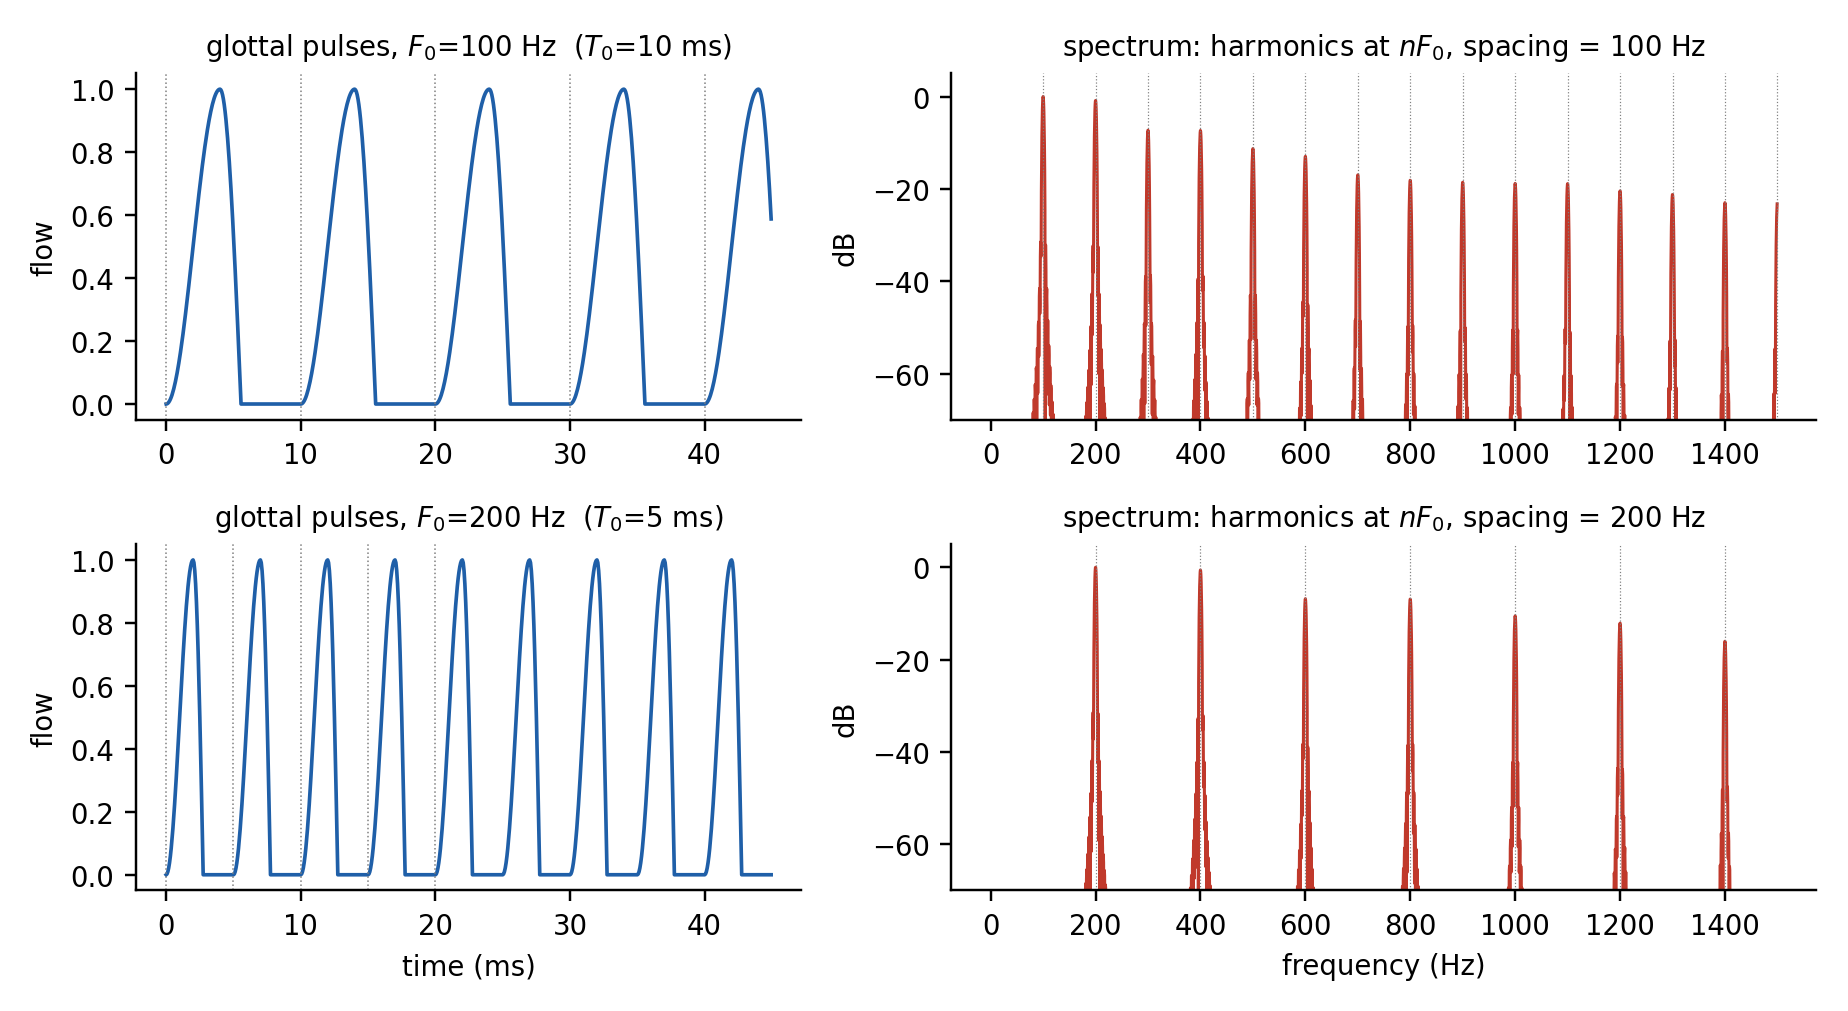
\includegraphics[width=0.95\textwidth]{../assets/figures/ch03-glottal-harmonics.png}
\caption{بالا: دنبالهٔ تپ‌های ساده‌شدهٔ هوای عبوری از چاکنای با $F_0=100$ هرتز و طیف آن. پایین: همان با $F_0=200$ هرتز. در هر دو مورد هارمونیک‌ها در مضارب صحیح $F_0$ ظاهر می‌شوند و فاصلهٔ آن‌ها دقیقاً $F_0$ است؛ دامنه با افزایش فرکانس به‌تدریج کاهش می‌یابد (شکل افزوده).}
\end{figure}

\subsection{فاصلهٔ هارمونیک‌ها و $F_0$}
فاصلهٔ فرکانسی دو هارمونیک متوالی برابر $F_n-F_{n-1}=F_0$ است. پس:
\begin{itemize}
  \item هرچه $F_0$ بزرگ‌تر (صدای زیرتر)، هارمونیک‌ها دورتر از هم‌اند؛
  \item هرچه $F_0$ کوچک‌تر (صدای بم‌تر)، هارمونیک‌ها فشرده‌تر و تعدادشان در یک بازهٔ ثابت بیشتر است.
\end{itemize}
به همین دلیل از فاصلهٔ خطوط هارمونیکی در اسپکتروگرام می‌توان $F_0$ و تغییرات آن (زیر و بمی) را خواند.

\begin{addedbox}{مثال عددی: تعداد هارمونیک‌ها}
در بازهٔ $0$ تا $4000$ هرتز:
\begin{itemize}
  \item برای $F_0=100$ هرتز: ${4000}/{100}=40$ هارمونیک؛
  \item برای $F_0=200$ هرتز: ${4000}/{200}=20$ هارمونیک.
\end{itemize}
بنابراین در صدای مردانه‌ای که $F_0$ پایین‌تری دارد، طیف «پرتراکم‌تر» است.
\end{addedbox}

\subsection{چرا کافی نیستند؟}
$F_0$ و هارمونیک‌ها نشان می‌دهند «منبع صدا» چگونه است، اما اینکه چرا «آ» با «ای» تفاوت دارد، با آن‌ها توضیح داده نمی‌شود. برای این به مدل منبع--فیلتر نیاز داریم؛ ولی ابتدا نمایشی از طیف در طول زمان می‌سازیم.

\section{اسپکتروگرام}

\subsection{از طیف به اسپکتروگرام}
تبدیل فوریهٔ کل گفتار، یک طیف واحد می‌دهد و اطلاعات زمانی را از دست می‌دهد؛ در حالی که گفتار ایستا نیست و اندام‌ها و محتوای فرکانسی دائم تغییر می‌کنند. \term{اسپکتروگرام}{Spectrogram} (طیف‌نگاره؛ از \eng{Spectro} برگرفته از \eng{Spectrum} یعنی طیف و \eng{Gram} یعنی نگاره یا ثبت) تغییرات محتوای فرکانسی را در طول زمان نمایش می‌دهد.

\subsection{مراحل ساخت}
\begin{enumerate}
  \item سیگنال به پنجره‌ها یا فریم‌های زمانی کوتاه (مثلاً ۲۵ میلی‌ثانیه) بریده می‌شود (\eng{Windowing}). پنجره‌ها ممکن است هم‌پوشانی (\eng{Overlap}) داشته باشند یا نداشته باشند.
  \item روی هر فریم تبدیل فوریه اعمال می‌شود و بزرگی طیف هر فریم به دست می‌آید.
  \item این طیف‌ها به‌ترتیب زمان کنار هم چیده می‌شوند و تصویر دوبعدی اسپکتروگرام را می‌سازند.
\end{enumerate}
این روش را \term{تبدیل فوریهٔ زمان-کوتاه}{Short-Time Fourier Transform, STFT} می‌نامند.

\begin{addedbox}{مثال عددی: تعداد فریم‌ها}
برای سیگنالی به طول $1$ ثانیه با $f_s=16000$ هرتز (یعنی $16000$ نمونه)، پنجره $25$ میلی‌ثانیه ($400$ نمونه) و گام $10$ میلی‌ثانیه ($160$ نمونه):
\[
\text{تعداد فریم‌ها}=1+\left\lfloor\frac{16000-400}{160}\right\rfloor=1+97=98.
\]
هر فریم یک ستون از اسپکتروگرام است؛ پس این اسپکتروگرام حدود ۹۸ ستون دارد.
\end{addedbox}

\subsection{محورها و رنگ}
در اسپکتروگرام:
\begin{itemize}
  \item محور افقی: زمان؛
  \item محور عمودی: فرکانس؛
  \item رنگ یا روشنایی هر نقطه: بزرگی (انرژی یا توان) آن مؤلفهٔ فرکانسی در آن لحظه.
\end{itemize}
به بیان تخته: اگر یک تصویر دوبعدی (زمان--دامنه) را به‌صورت فضای سه‌بعدی ببینیم، محور سوم همان فرکانس است و دامنه به شکل رنگ پیکسل‌ها نمایش داده می‌شود. رنگ گرم یعنی بزرگی بالا، یعنی آن فرکانس شباهت زیادی با سیگنال ورودی داشته و معمولاً هارمونیک صدای ورودی است؛ رنگ سرد یعنی بزرگی پایین و شباهت اندک.

\boardfigure{0.7}{ch03-board-spectrogram-harmonics.png}{اسپکتروگرام یک صدای تقریباً پایدار با رنگ‌گذاری گرم/سرد: خطوط افقی پررنگ، هارمونیک‌ها هستند و با گذر زمان کمی تغییر می‌کنند. مقیاس محور فرکانس در این تصویر مربوط به همان نمونهٔ منبع است.}

\begin{correctionbox}{مقیاس رنگ معمولاً دسی‌بل است}
در اسپکتروگرام‌های رایج، رنگ نشان‌دهندهٔ لگاریتم بزرگی (دسی‌بل: $20\log_{10}|X|$) است، نه خود بزرگی؛ چرا که دامنهٔ هارمونیک‌های قوی و ضعیف چندین مرتبه با هم فرق دارد و در مقیاس خطی مؤلفه‌های ضعیف دیده نمی‌شوند. همچنین اسپکتروگرام معمولاً فقط بزرگی را نشان می‌دهد و فاز کنار گذاشته می‌شود.
\end{correctionbox}

\begin{warningbox}{فرکانس و دامنه دو چیز متفاوت‌اند}
فرکانس می‌گوید موج با چه سرعتی نوسان می‌کند و دامنه می‌گوید اندازهٔ نوسان چقدر است. قرار داشتن یک مؤلفه در فرکانس بالاتر به این معنی نیست که دامنهٔ بیشتری دارد. این تمایز در پرسش و پاسخ‌های کلاس چند بار مورد تأکید قرار گرفت. در اسپکتروگرام، «ارتفاع» روی محور عمودی \emph{فرکانس} است و «پررنگی» \emph{دامنه}.
\end{warningbox}

\section{مدل منبع--فیلتر}

\subsection{مسئلهٔ حل‌نشده}
با $F_0$ و هارمونیک‌ها فقط می‌توانیم «منبع» را بشناسیم. اما وقتی فردی از «آ» به «ای» می‌رود، $F_0$ را ثابت نگه دارد و فقط شکل دهان و موقعیت زبان را عوض کند، صدا فرق می‌کند. این تغییر از $F_0$ نمی‌آید. پس مدل کامل‌تری لازم است.

\begin{definitionbox}{مدل منبع--فیلتر (\lr{Source--Filter})}
تولید گفتار به دو بخش مستقل (در تقریب مدل) تقسیم می‌شود:
\begin{itemize}
  \item \textbf{منبع (\lr{Source}):} برای صداهای واک‌دار، ارتعاش تارهای صوتی که موجی دوره‌ای با فرکانس پایه و هارمونیک‌های آن تولید می‌کند؛
  \item \textbf{فیلتر (\lr{Filter}):} مجرای صوتی (\eng{Vocal Tract}) که بسته به شکلش بخش‌هایی از طیف را تقویت (تشدید) و بخش‌هایی را تضعیف می‌کند.
\end{itemize}
\end{definitionbox}

در حوزهٔ فرکانس، خروجی حاصل‌ضرب طیف منبع در پاسخ فرکانسی فیلتر است (همان فرمولی که روی تخته نوشته شد):
\[
\text{\lr{Output}}(f)=\text{\lr{Source}}(f)\times\text{\lr{Filter}}(f).
\]
در حوزهٔ زمان، این عمل یک \term{کانولوشن}{Convolution} است و اگر لگاریتم بگیریم، ضرب به جمع تبدیل می‌شود: $\log|\text{Out}|=\log|\text{Src}|+\log|\text{Filt}|$ (در شکل زیر هم همین است).

\boardfigure{0.85}{ch03-board-source-filter.png}{نمودار ورودی (طیف منبع در تارهای صوتی با هارمونیک‌های کاهنده)، فیلتر (پاسخ فرکانسی مجرای صوتی با قله‌های تشدیدی) و خروجی (طیف هارمونیک‌ها که بر اساس شکل فیلتر قله و درّه یافته است).}

\begin{figure}[htbp]
\centering
\begin{tikzpicture}[rtl, node distance=1.2cm, every node/.style={font=\small},
  box/.style={draw, rounded corners, minimum width=2.8cm, minimum height=1.1cm, align=center},
  arr/.style={-{Stealth[length=2.5mm]}, thick}]
  \node[box, fill=blue!10] (src) {منبع\\ \lr{Source}\\ \footnotesize تارهای صوتی};
  \node[box, left=of src, fill=green!10] (fil) {فیلتر\\ \lr{Filter}\\ \footnotesize مجرای صوتی};
  \node[box, left=of fil, fill=orange!12] (out) {خروجی\\ \lr{Output}\\ \footnotesize موج گفتار};
  \draw[arr] (src) -- (fil); \draw[arr] (fil) -- (out);
  \node[below=0.5mm of src, font=\scriptsize, align=center] {\lr{$F_0$ and harmonics}};
  \node[below=0.5mm of fil, font=\scriptsize, align=center] {\lr{formants $F_1,F_2,F_3$}};
  \node[below=0.5mm of out, font=\scriptsize, align=center] {\lr{harmonics shaped by formants}};
\end{tikzpicture}
\caption{نمای ساده‌شدهٔ مدل منبع--فیلتر برای صداهای واک‌دار (شکل افزوده).}
\end{figure}

\subsection{مجرای صوتی به‌مثابهٔ لوله}
استاد برای سادگی مجرای صوتی را شبیه یک لوله در نظر گرفتند که هر تغییر شکلش بر موجِ عبوری اثر می‌گذارد. عواملی که شکل این فیلتر را تغییر می‌دهند: موقعیت زبان، میزان باز بودن دهان، موقعیت فک، وضعیت لب‌ها و محل تنگ‌شدگی در مسیر هوا. وقتی هنگام صحبت اندام‌ها را حرکت می‌دهیم، در واقع مشخصات فیلتر را تغییر می‌دهیم.

\boardfigure{0.75}{ch03-board-tube-model.png}{مدل لوله‌ای ساده از مجرای صوتی: لوله‌ای به طول حدود $17.5$ سانتی‌متر که در سمت چاکنای (تارهای صوتی) بسته و در سمت لب‌ها باز است؛ سطح مقطع حدود ۱ سانتی‌متر مربع.}

\begin{addedbox}{مثال عددی: فرمنت‌های یک لولهٔ یک‌سر‌بسته}
برای لوله‌ای به طول $L$ که یک سر بسته (چاکنای) و یک سر باز (لب) دارد، فرکانس‌های تشدید برابرند با:
\[
F_n=\frac{(2n-1)\,c}{4L},\qquad n=1,2,3,\dots
\]
که $c\approx 350$ متر بر ثانیه سرعت صوت در هوای گرم دهان است. برای $L=17.5$ سانتی‌متر:
\[
F_1=\frac{35000}{4\times17.5}=500,\qquad F_2=1500,\qquad F_3=2500\ \text{هرتز.}
\]
این مجموعه تقریباً فرمنت‌های یک واکهٔ خنثی (شبیه \eng{schwa}) است. برای مجرای کوتاه‌تر با $L=15$ سانتی‌متر: $F_1\approx 583,\ F_2\approx 1750,\ F_3\approx 2917$ هرتز؛ یعنی فرمنت‌ها حدود ۱۷ درصد بالاتر می‌روند. این توضیح می‌دهد چرا فرمنت‌های گویندگان با مجرای کوتاه‌تر (زنان و کودکان) بالاتر است.
\end{addedbox}

\subsection{کار فیلتر: تشدید و تضعیف}
مهم‌ترین نقش فیلتر، تقویت (تشدید) و تضعیف نواحی مختلف طیف است. منبع مجموعه‌ای از هارمونیک‌ها تولید می‌کند و با تغییر شکل دهان، بعضی هارمونیک‌ها تقویت و بعضی تضعیف می‌شوند. این همان پیوندی است که از ابتدای جلسه دنبال می‌کردیم: تغییر وضعیت اندام‌ها $\leftarrow$ تغییر قابل مشاهده در طیف موج.

\begin{figure}[htbp]
\centering
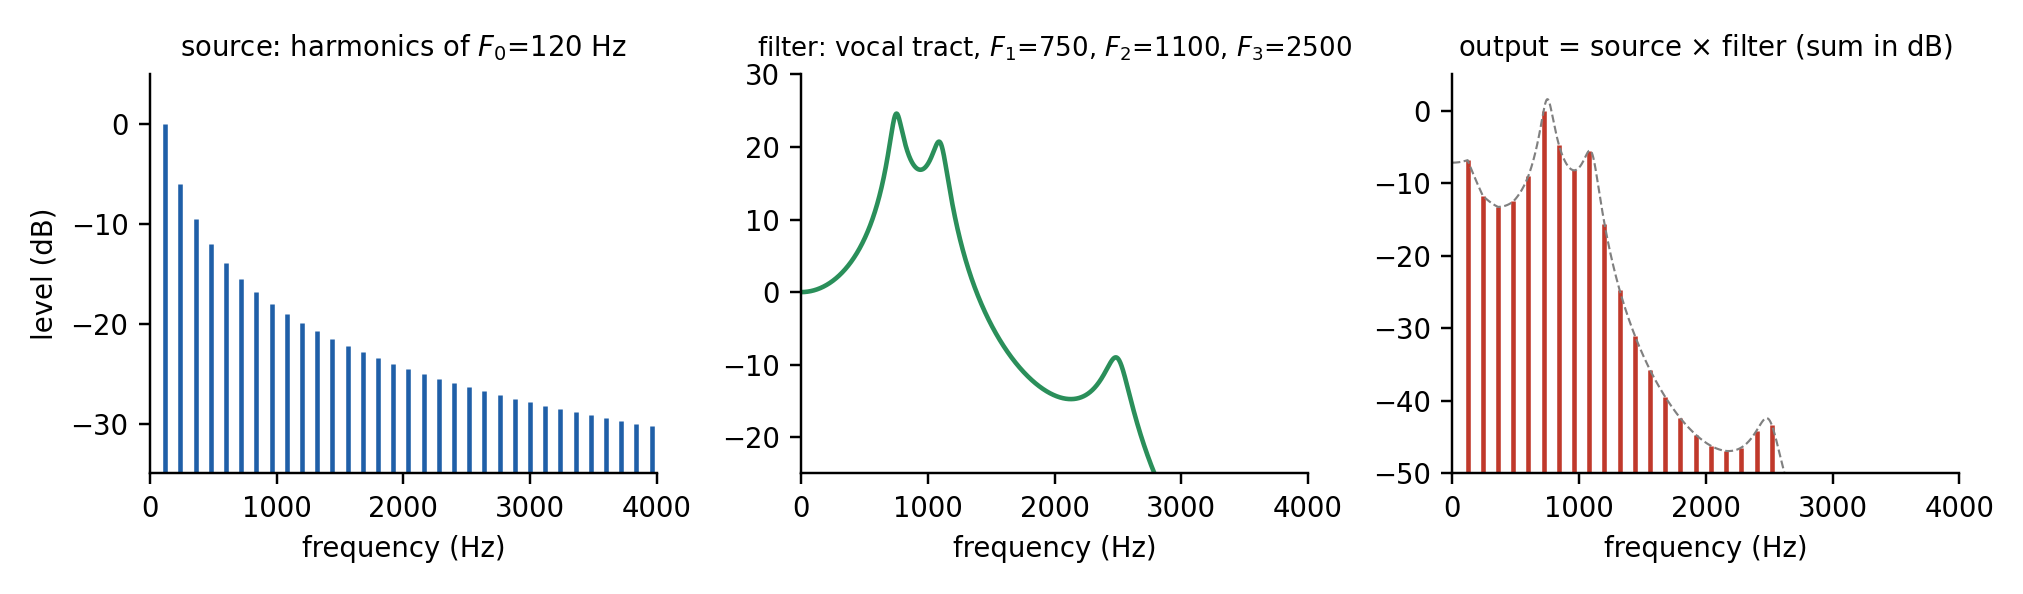
\includegraphics[width=0.95\textwidth]{../assets/figures/ch03-source-filter-spectra.png}
\caption{نمونهٔ عددی مدل منبع--فیلتر با $F_0=120$ هرتز: (الف) هارمونیک‌های منبع با افت تدریجی دامنه؛ (ب) پاسخ فرکانسی مجرا با فرمنت‌های $F_1=750$، $F_2=1100$ و $F_3=2500$ هرتز؛ (ج) خروجی که از جمع دو منحنی در مقیاس دسی‌بل به دست می‌آید. خط‌چین، پوش طیفی خروجی را نشان می‌دهد و هارمونیک‌ها نمونه‌هایی از همین پوش‌اند (شکل افزوده).}
\end{figure}

\begin{correctionbox}{وضعیت دقیق «استقلال» منبع و فیلتر}
مدل منبع--فیلتر یک تقریب است: فرض می‌کند منبع و فیلتر تقریباً مستقل‌اند، یعنی تغییر $F_0$ فرمنت‌ها را جابه‌جا نمی‌کند و تغییر شکل مجرا، $F_0$ را عوض نمی‌کند. این فرض برای بیشتر تحلیل‌ها خوب کار می‌کند و به همین دلیل می‌توانیم در سیگنال خروجی $F_0$ را از فرمنت‌ها جدا بخوانیم. در واقعیت بازتاب‌هایی میان مجرا و چاکنای (برهم‌کنش منبع و مجرا) و اثر تابش از لب‌ها نیز وجود دارد که در مدل ساده نادیده گرفته می‌شود. در نمودار منبع، افت هارمونیک‌ها حدود ۱۲ دسی‌بل بر اکتاو است (شکل ناشی از تپ‌های هوای چاکنای) و تابش از لب‌ها حدود ۶ دسی‌بل بر اکتاو آن را جبران می‌کند؛ در شکل افزودهٔ بالا برای سادگی فقط شیب نهایی (حدود $-6$ دسی‌بل بر اکتاو) رسم شده است.
\end{correctionbox}

\subsection{آیا همهٔ صداها از تارهای صوتی می‌آیند؟}
خیر. همخوان‌های بی‌واک مانند «س» بدون ارتعاش تارهای صوتی تولید می‌شوند. در آن‌ها منبع، \emph{نویز آشفتگی} جریان هوا در یک تنگنا است (نه سری از تپ‌های متناوب)، پس هارمونیک ندارند و طیف آن‌ها پیوسته است. فیلتر مجرای صوتی (بخش جلوی تنگنا) همچنان طیف این نویز را شکل می‌دهد. بنابراین مدل «منبع = ارتعاش تارها» تنها برای صداهای واک‌دار است و تمرکز این جلسه هم بر همین حالت بود.

\section{فرمنت‌ها}

\subsection{تعریف}
\begin{definitionbox}{فرمنت (\lr{Formant})}
فرمنت‌ها نواحی تشدید مجرای صوتی هستند؛ نواحی از فرکانس که فیلتر آن‌ها را تقویت می‌کند. در طیف، فرمنت به‌صورت یک قلهٔ پهن در پوش طیف و در اسپکتروگرام باند پهن به‌صورت نوار یا توده‌ای پررنگ دیده می‌شود.
\end{definitionbox}

نکتهٔ مهم: فرمنت یک هارمونیک منفرد نیست؛ یک \emph{ناحیهٔ} فرکانسی است که دامنهٔ چند هارمونیک مجاور را هم‌زمان بالا می‌برد. فرمنت‌ها مربوط به فیلتر هستند: مجرای صوتی خواص تشدیدی خود را دارد، چه منبع در حال تحریک باشد و چه نباشد. همچنین ما هنگام تحلیل، فرمنت‌ها را \emph{نمی‌سازیم}؛ آن‌ها نتیجهٔ تشدیدهای مجرا هستند و در تحلیل، اثرشان را روی موج شناسایی می‌کنیم.

\subsection{فرمنت اول، دوم و سوم}
فرمنت‌ها بر اساس ترتیب فرکانسی نام‌گذاری می‌شوند:
\[
F_1<F_2<F_3<F_4<\cdots
\]
یعنی $F_1$ پایین‌ترین ناحیهٔ تشدیدی است (در اسپکتروگرام از فرکانس‌های پایین شروع می‌کنیم و اولین ناحیهٔ تشدیدی را $F_1$ می‌نامیم). این ترتیب، ترتیب فرکانسی است و ربطی به ترتیب زمانی تولید ندارد.

\subsection{ارتباط فرمنت‌ها با نقشهٔ واکه‌ها}
مهم‌ترین ارتباط جلسه این است که همان ویژگی‌های نقشهٔ واکه‌ها که جلسهٔ پیش دیدیم، در موقعیت فرمنت‌ها دیده می‌شوند:

\begin{center}
\begin{tabular}{ll}
\toprule
ویژگی تولیدی & ویژگی آکوستیکی مرتبط \\
\midrule
ارتفاع زبان / میزان بازشدگی دهان & $F_1$ \\
جلو یا عقب بودن زبان & $F_2$ \\
\bottomrule
\end{tabular}
\end{center}

\begin{itemize}
  \item \textbf{$F_1$:} برای واکه‌های بازتر (زبان پایین‌تر، دهان بازتر) بالاتر و برای واکه‌های بسته‌تر پایین‌تر است. «آ» $F_1$ بالاتری از «ای» دارد.
  \item \textbf{$F_2$:} برای واکه‌های جلویی بالاتر و برای واکه‌های عقبی پایین‌تر است.
\end{itemize}
در تخته توضیحی نیز نوشته شده بود: وقتی زبان به جلو می‌آید، محفظهٔ جلوی دهان کوچک‌تر می‌شود و $F_2$ بالا می‌رود؛ و تنگ‌شدن محفظهٔ حلق (مانند «آ») $F_1$ را بالا می‌برد.

\boardfigure{0.9}{ch03-board-vowel-tract-spectra.png}{برای سه واکهٔ \eng{i}، \eng{a} و \eng{u}: برش مجرای صوتی (چپ)، مدل لوله‌ای ساده آن (وسط) و طیف آکوستیکی یا پاسخ فرکانسی فیلتر (راست). با تغییر شکل مجرا، قله‌های تشدیدی (فرمنت‌ها) جابه‌جا می‌شوند.}

\boardfigure{0.8}{ch03-board-formants-iau.png}{اسپکتروگرام سه واکهٔ \eng{/i/}، \eng{/a/} و \eng{/u/} با خطوط افقی که موقعیت $F_1$ تا $F_3$ را نشان می‌دهند. در \eng{/i/} فاصلهٔ $F_1$ و $F_2$ بسیار زیاد است؛ در \eng{/a/} فرمنت اول بالاتر از دو واکهٔ دیگر است؛ در \eng{/u/} هر دو فرمنت اول و دوم پایین‌اند.}

\begin{addedbox}{مقادیر نوعی فرمنت واکه‌ها (مردان بالغ، تقریبی)}
\begin{center}
\begin{tabular}{lccc}
\toprule
واکه & $F_1$ (هرتز) & $F_2$ (هرتز) & $F_3$ (هرتز) \\
\midrule
\eng{/i/} (مانند «ای») & $270$ & $2290$ & $3010$ \\
\eng{/a/} (مانند «آ») & $730$ & $1090$ & $2440$ \\
\eng{/u/} (مانند «او») & $300$ & $870$ & $2240$ \\
\bottomrule
\end{tabular}
\end{center}
این اعداد میانگین‌های واکه‌های انگلیسی مطالعهٔ کلاسیک پترسون و بارنی (۱۹۵۲) هستند و فقط برای نشان‌دادن الگو آورده شده‌اند؛ مقادیر واکه‌های فارسی و گویندگان مختلف کمی فرق دارد. الگوی کلی مطابق کلاس است: $F_1$ در «ای» و «او» کم و در «آ» زیاد، و $F_2$ در «ای» خیلی بالا و در «او» پایین است.
\end{addedbox}

\begin{figure}[htbp]
\centering
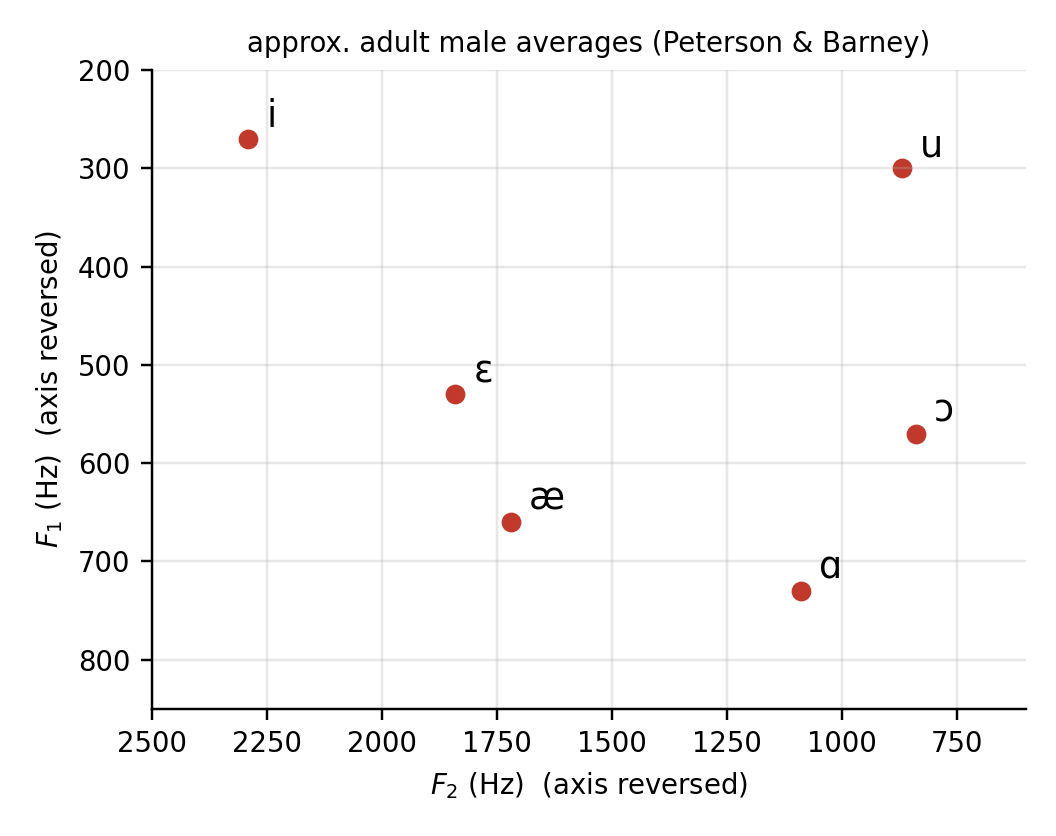
\includegraphics[width=0.6\textwidth]{../assets/figures/ch03-vowel-f1f2.png}
\caption{نقشهٔ آکوستیکی واکه‌ها در صفحهٔ $F_1$--$F_2$ (با محورهای معکوس). این نمودار شبیه نقشهٔ واکه‌ها در آواشناسی تولیدی است: واکه‌های جلویی و بسته بالا و چپ، واکه‌های بازتر پایین‌تر، و واکه‌های عقبی سمت راست قرار می‌گیرند (شکل افزوده).}
\end{figure}

\subsection{فرمنت‌ها و طول مجرای صوتی}
طول مجرای صوتی (که ویژگی فیلتر است، نه منبع) بر محدودهٔ فرکانسی فرمنت‌ها اثر دارد: هرچه مجرا بلندتر، فرمنت‌ها پایین‌تر (به سمت فرکانس‌های بم‌تر) می‌روند و هرچه کوتاه‌تر، فرمنت‌ها بالاتر می‌روند. معمولاً مجرای مردان بلندتر است. این یکی از دلایلی است که $F_0$ به‌تنهایی جنسیت را مشخص نمی‌کند.

\boardfigure{0.75}{ch03-board-voices-formants.png}{اسپکتروگرام یک واکه برای سه نسخه از صدا: مردانه‌شده، نمونه، و زنانه‌شده. با حرکت از صدای مردانه به زنانه، فرمنت‌های $F_1$ تا $F_4$ به سمت فرکانس‌های بالاتر جابه‌جا می‌شوند.}

\subsection{هارمونیک در برابر فرمنت}
\begin{center}
\begin{tabular}{p{2.8cm}p{5cm}p{5.5cm}}
\toprule
ویژگی & هارمونیک (\eng{Harmonic}) & فرمنت (\eng{Formant}) \\
\midrule
منشأ اصلی & تناوب منبع صوتی (تارها) & تشدیدهای مجرای صوتی \\
نوع نمایش & مؤلفه‌ای در فرکانس مشخص & ناحیه یا قلهٔ تشدیدی در پوش طیف \\
ارتباط با $F_0$ & مضارب صحیح $F_0$ & لزوماً مضرب صحیح $F_0$ نیست \\
کاربرد در بحث & بررسی ساختار منبع و \eng{Pitch} & بررسی ویژگی‌های تولیدی و واکه‌ها \\
\bottomrule
\end{tabular}
\end{center}

\begin{addedbox}{مثال عددی: کدام هارمونیک‌ها تقویت می‌شوند؟}
فرض کنید $F_0=120$ هرتز و $F_1=750$ هرتز باشد. هارمونیک‌ها عبارت‌اند از:
\begin{center}
\begin{tabular}{c|cccccccc}
\toprule
$n$ & 1 & 2 & 3 & 4 & 5 & 6 & 7 & 8\\
\midrule
$nF_0$ (هرتز) & 120 & 240 & 360 & 480 & 600 & 720 & 840 & 960\\
\bottomrule
\end{tabular}
\end{center}
فاصلهٔ آن‌ها تا $750$ هرتز: $H_6$: $30$، $H_7$: $90$، $H_5$: $150$، $H_8$: $210$ هرتز. پس هارمونیک‌های ششم و هفتم (۷۲۰ و ۸۴۰) بیشترین تقویت را می‌گیرند و ششم از همه به فرمنت نزدیک‌تر است. میزان دقیق تقویت به شکل و پهنای قلهٔ تشدیدی بستگی دارد؛ همین است که فرمنت در اسپکتروگرام یک ناحیهٔ پررنگ است، نه یک خط. این همان مثالی است که روی تخته با فهرست $120,240,\dots,1320$ هرتز بررسی شد (شکل \ref{fig:ch03-harmonics-f1}).
\end{addedbox}

\begin{figure}[htbp]
\centering
\begin{tikzpicture}[rtl, x=1cm,y=1cm,scale=1]
\def\u{0.0088}% cm per Hz
\fill[softblue] plot[smooth,domain=0:1340,samples=60] (\u*\x,{0.1+2.0*exp(-((\x-750)/230)^2)}) -- (\u*1340,0) -- (0,0) -- cycle;
\draw[mainblue, thick, smooth, domain=0:1340, samples=60, variable=\x] plot (\u*\x,{0.1+2.0*exp(-((\x-750)/230)^2)});
\foreach \n in {1,...,11}{
  \pgfmathtruncatemacro{\f}{120*\n}
  \pgfmathsetmacro{\h}{0.1+2.0*exp(-((\f-750)/230)^2)}
  \ifnum\n=6 \def\c{red!75!black}\def\w{1.8pt}\else\ifnum\n=7 \def\c{red!75!black}\def\w{1.8pt}\else\def\c{black!65}\def\w{0.9pt}\fi\fi
  \draw[\c, line width=\w] (\u*\f,0) -- (\u*\f,\h);
  \node[font=\scriptsize, below=1pt] at (\u*\f,0) {\lr{\n}};
  \node[font=\scriptsize, below=11pt, text=black!70] at (\u*\f,0) {\lr{\f}};
}
\draw[-{Stealth[length=2mm]}, thick] (0,0) -- (\u*1400,0) node[right, font=\small] {\lr{Hz}};
\draw[dashed, red!75!black] (\u*750,0) -- (\u*750,2.65);
\node[above, font=\small, red!75!black] at (\u*750,2.65) {\lr{$F_1=750$ Hz}};
\node[font=\scriptsize, anchor=east] at (-0.15,-0.2) {شماره};
\node[font=\scriptsize, anchor=east, text=black!70] at (-0.15,-0.62) {\lr{$nF_0$}};
\end{tikzpicture}
\caption{مثال تخته: با $F_0=120$ هرتز و $F_1=750$ هرتز، هارمونیک‌ها در ۱۲۰، ۲۴۰، ۳۶۰، \dots هرتز قرار دارند و شمارهٔ هرکدام زیر آن نوشته شده است. هارمونیک‌های نزدیک به قلهٔ تشدیدی (ششم و هفتم، ۷۲۰ و ۸۴۰ هرتز، با رنگ قرمز) بیشترین تقویت را می‌گیرند؛ منحنی آبی شکل کلی فیلتر مجرای صوتی است (منحنی افزوده) (بازسازی‌شده از تختهٔ کلاس).}
\label{fig:ch03-harmonics-f1}
\end{figure}

\section{اسپکتروگرام باند باریک و باند پهن}

\subsection{مبادله میان وضوح زمانی و فرکانسی}
کلید فهم دو نوع اسپکتروگرام، یک مبادله (\eng{trade-off}) بنیادی است:
\begin{itemize}
  \item پنجرهٔ \textbf{کوتاه}: تغییرات سریع در زمان بهتر دیده می‌شوند، اما توان تفکیک فرکانس‌های نزدیک کم می‌شود.
  \item پنجرهٔ \textbf{بلند}: فرکانس‌های نزدیک بهتر تفکیک می‌شوند، اما تغییرات سریع زمانی محو می‌شوند.
\end{itemize}
وضوح فرکانسی تقریباً با معکوس طول پنجره متناسب است ($\Delta f\sim 1/L$).

\begin{definitionbox}{باند پهن در برابر باند باریک}
\textbf{باند پهن (\lr{Wideband}):} پنجرهٔ کوتاه، حدود ۳ تا ۵ میلی‌ثانیه (استاد مثال ۵ میلی‌ثانیه زدند). وضوح زمانی بالا، وضوح فرکانسی پایین؛ هارمونیک‌ها در هم ادغام می‌شوند و بیشتر پوش طیفی، یعنی فرمنت‌ها، دیده می‌شود.

\textbf{باند باریک (\lr{Narrowband}):} پنجرهٔ بلندتر، حدود ۲۰ تا ۵۰ میلی‌ثانیه (در ابزار کلاس ۳۰ میلی‌ثانیه). وضوح فرکانسی بالا، وضوح زمانی پایین؛ هارمونیک‌ها به‌صورت خطوط افقی باریک و مجزا دیده می‌شوند.
\end{definitionbox}

\begin{center}
\begin{tabular}{lcc}
\toprule
ویژگی & باند پهن & باند باریک \\
\midrule
طول پنجره & کوتاه & بلند \\
وضوح زمانی & بالا & پایین \\
وضوح فرکانسی & پایین & بالا \\
نمایش مناسب‌تر & فرمنت‌ها & هارمونیک‌ها \\
\bottomrule
\end{tabular}
\end{center}

نکتهٔ مهم استاد: این دو نوع اسپکتروگرام مربوط به دو سیگنال متفاوت نیستند؛ هر دو از \emph{یک} سیگنال با تفاوت تنظیم پنجره ساخته می‌شوند. به بیان تخته: اگر دقت زمانی (رزولوشن زمانی) می‌خواهیم و به فرمنت‌ها علاقه‌مندیم $\Leftarrow$ \eng{wideband}؛ اگر دقت زمانی را قربانی می‌کنیم و رزولوشن فرکانسی (هارمونیک‌ها) می‌خواهیم $\Leftarrow$ \eng{narrowband}.

\begin{addedbox}{مثال عددی: پهنای باند تحلیل}
پهنای باند مؤثر یک پنجرهٔ هان تقریباً $1.5/L$ است. اگر $F_0=120$ هرتز:
\begin{itemize}
  \item پنجره $4$ میلی‌ثانیه: $1.5/0.004\approx 375$ هرتز. از آنجا که از فاصلهٔ هارمونیک‌ها (۱۲۰ هرتز) بیشتر است، هارمونیک‌ها در هم می‌روند. فقط پوش (فرمنت) می‌ماند. چون پنجره از یک دورهٔ تناوب ($8.3$ میلی‌ثانیه) کوتاه‌تر است، هر تپ چاکنایی جداگانه دیده می‌شود (خطوط عمودی).
  \item پنجره $32$ میلی‌ثانیه: $1.5/0.032\approx 47$ هرتز. این از ۱۲۰ هرتز کمتر است، پس هر هارمونیک جداگانه دیده می‌شود. این پنجره حدود ۴ دورهٔ تناوب را پوشش می‌دهد.
\end{itemize}
قاعدهٔ سرانگشتی: برای باند باریک پنجره باید چند دورهٔ تناوب $T_0$ را بپوشاند و برای باند پهن حدود یک دوره یا کمتر.
\end{addedbox}

\begin{figure}[htbp]
\centering
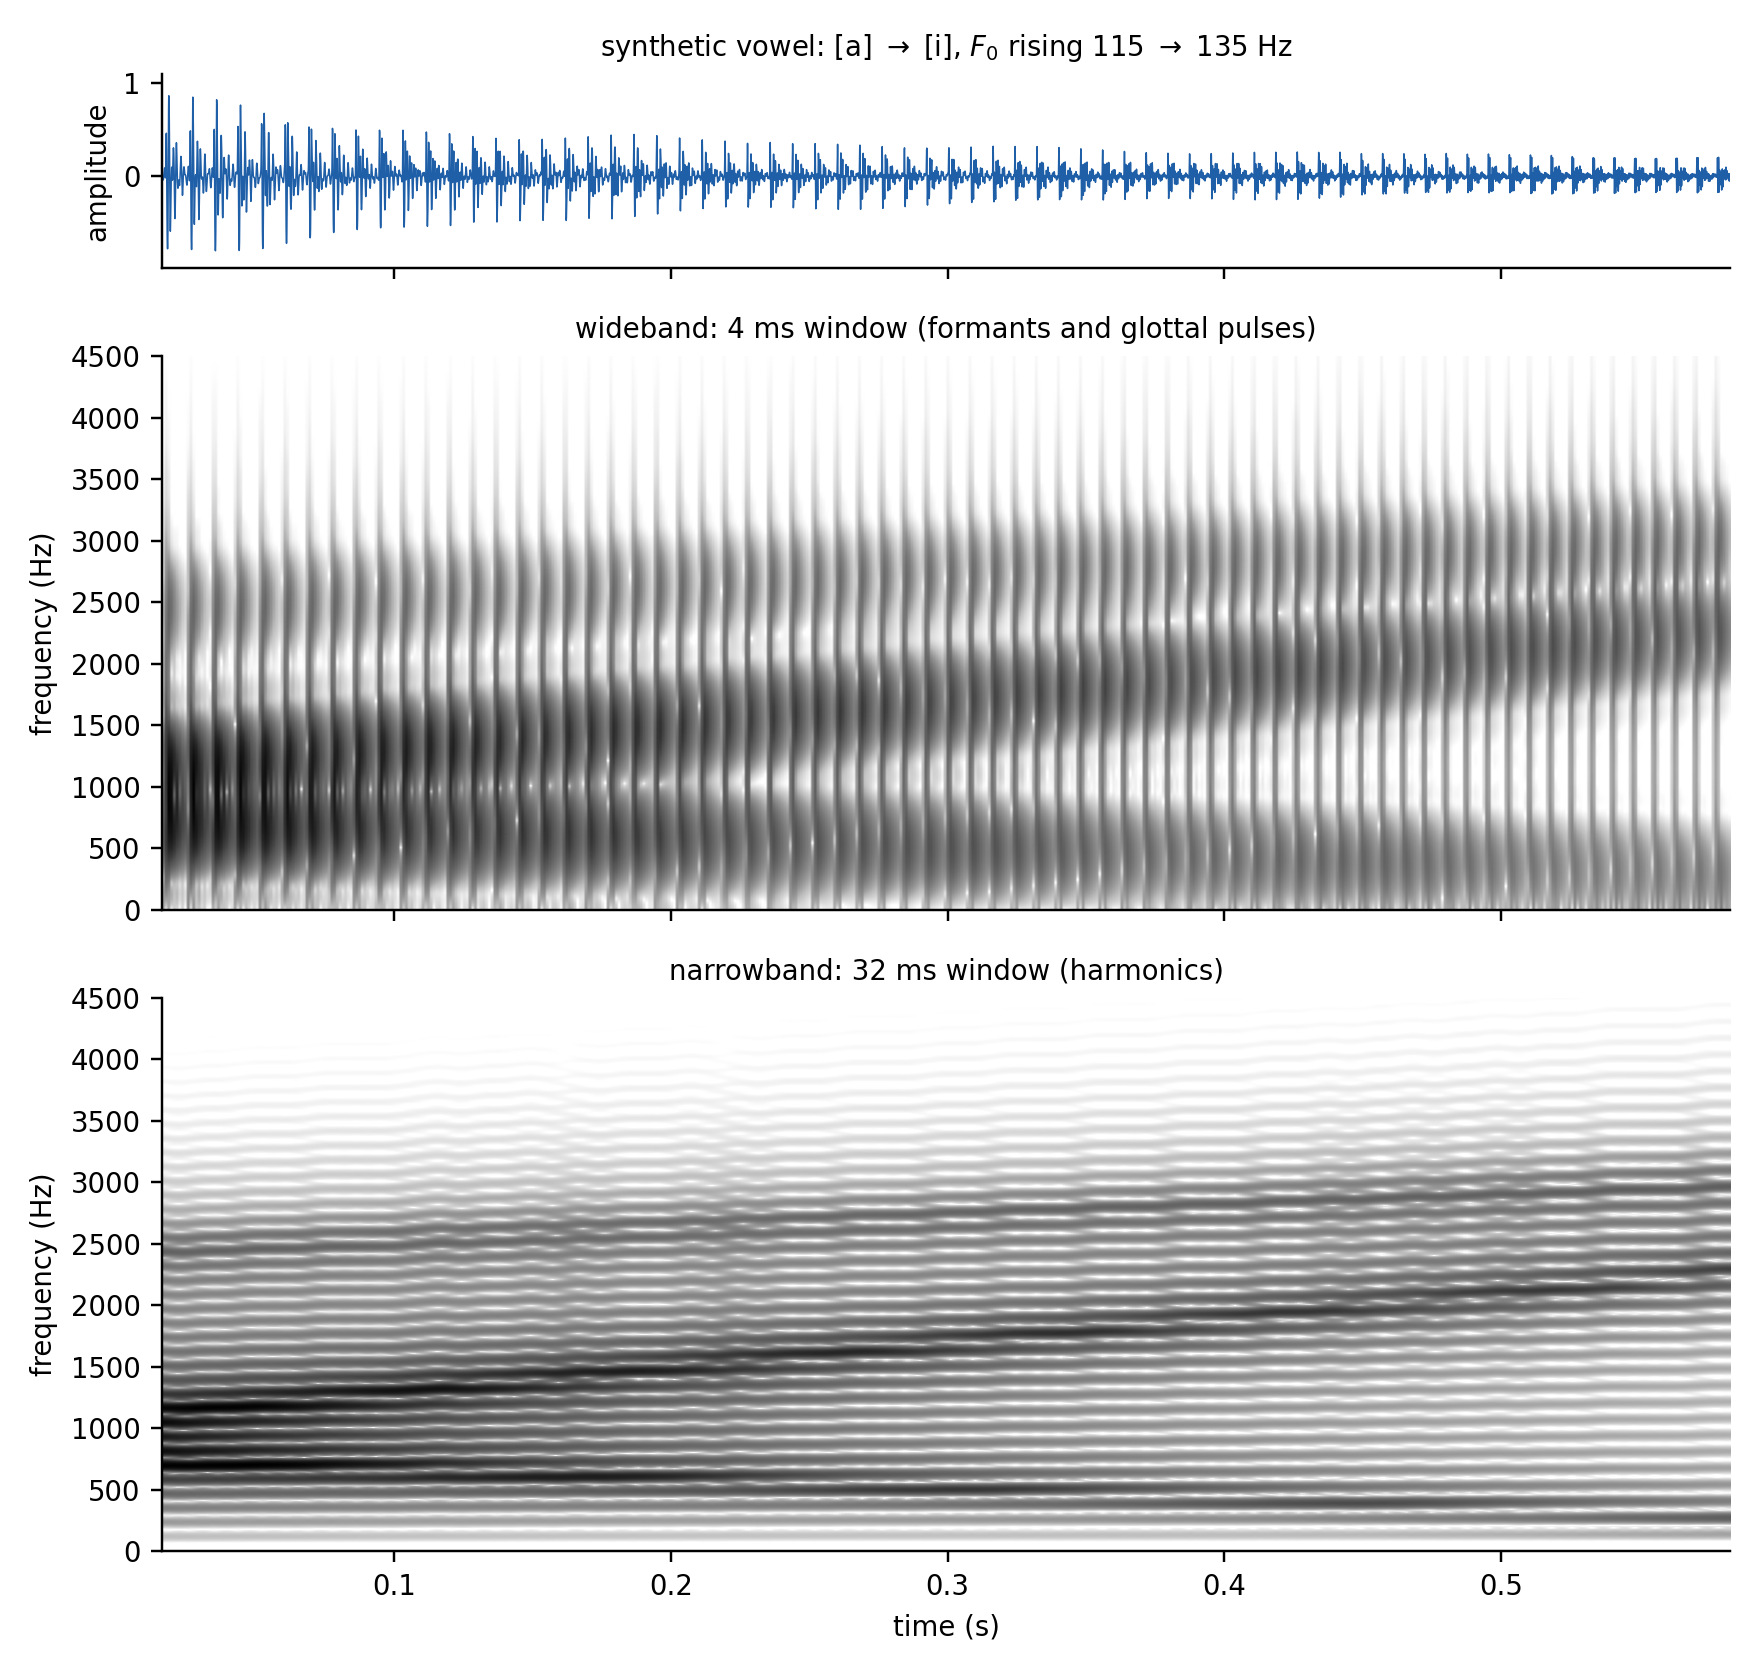
\includegraphics[width=0.95\textwidth]{../assets/figures/ch03-wideband-narrowband.png}
\caption{اسپکتروگرام باند پهن (پنجرهٔ ۴ میلی‌ثانیه) و باند باریک (پنجرهٔ ۳۲ میلی‌ثانیه) از \emph{یک} واکهٔ ترکیبی که به‌تدریج از «آ» به «ای» می‌رود و $F_0$ آن اندکی بالا می‌رود. باند پهن نوارهای فرمنتی ($F_1$ پایین‌رونده، $F_2$ بالارونده) و خطوط عمودی تپ‌های چاکنایی را نشان می‌دهد؛ باند باریک خطوط افقی هارمونیک‌ها را نشان می‌دهد که با افزایش $F_0$ اندکی شیب می‌گیرند (شکل افزوده).}
\end{figure}

\begin{figure}[htbp]
\centering
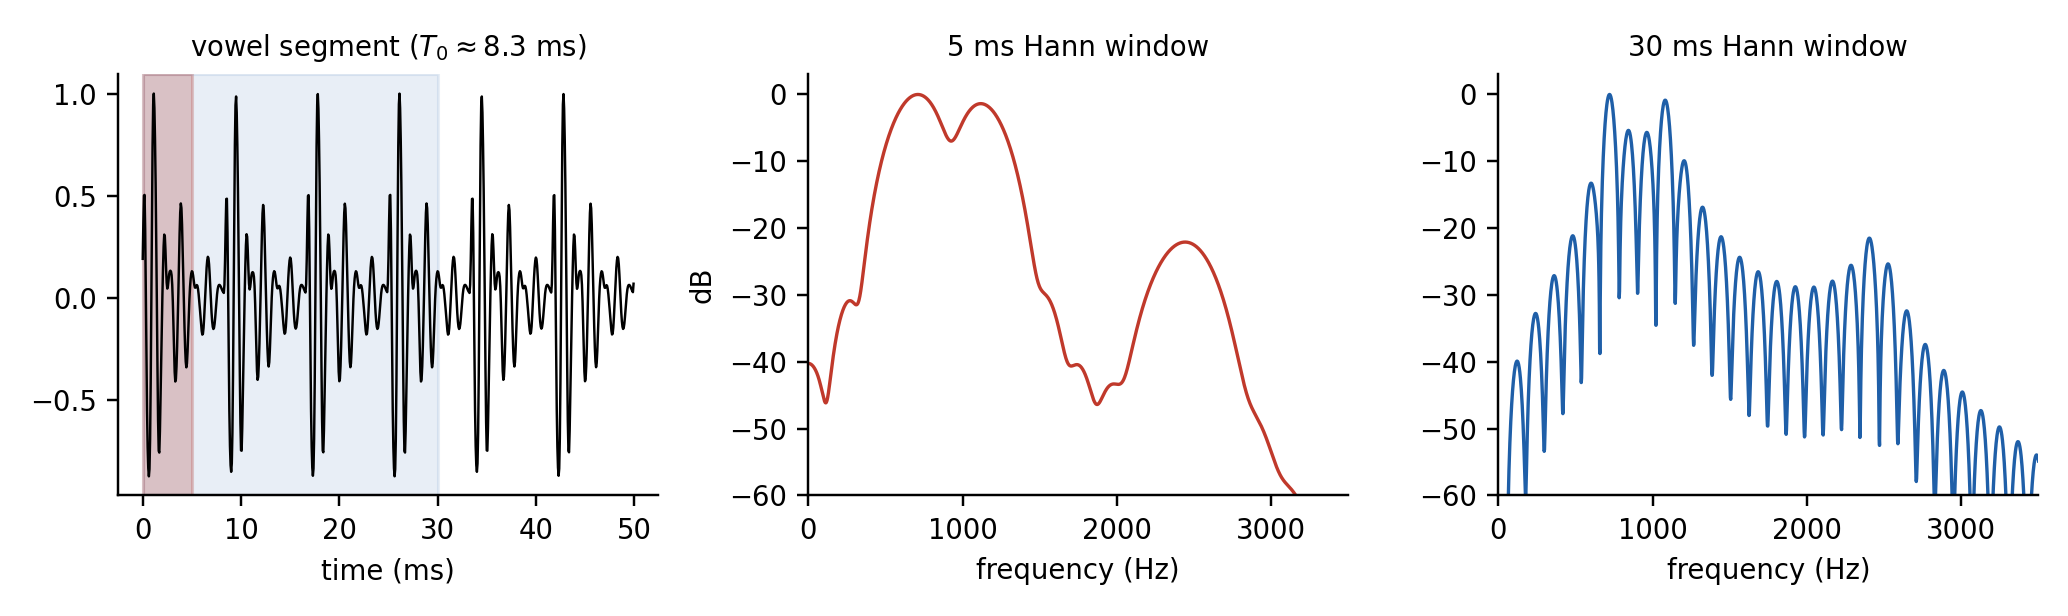
\includegraphics[width=0.95\textwidth]{../assets/figures/ch03-window-spectra.png}
\caption{طیف یک فریم از یک واکهٔ پایدار ($F_0=120$ هرتز) با دو طول پنجره. چپ: بخش‌هایی از موج که توسط پنجره‌ها پوشانده می‌شوند. وسط: پنجرهٔ ۵ میلی‌ثانیه که هارمونیک‌ها را محو و فقط پوش فرمنتی را نشان می‌دهد. راست: پنجرهٔ ۳۰ میلی‌ثانیه که هارمونیک‌ها را مجزا نشان می‌دهد (شکل افزوده).}
\end{figure}

\boardfigure{0.65}{ch03-board-wb-nb-tool.png}{خروجی ابزار پایتونی کلاس برای یک کلمه: زبانهٔ باند پهن (پنجرهٔ ۵ میلی‌ثانیه، مناسب فرمنت‌ها) و زبانهٔ باند باریک (پنجرهٔ ۳۰ میلی‌ثانیه، مناسب هارمونیک‌ها). بالا شکل موج و پایین اسپکتروگرام است.}

\subsection{چرا باند پهن برای فرمنت‌ها مناسب‌تر است؟}
فرمنت‌ها با تغییر وضعیت زبان و دهان تغییر می‌کنند و این تغییرات در بازه‌های بسیار کوتاه رخ می‌دهد؛ پس برای ردگیری آن‌ها وضوح زمانی خوب لازم است. در باند پهن علاوه بر این، به‌دلیل ادغام هارمونیک‌ها، پوش فرمنتی به‌صورت نوار پیوسته دیده می‌شود. در باند باریک تمرکز بر تفکیک دقیق هارمونیک‌هاست.

\section{پرسش و پاسخ}

\begin{description}[leftmargin=0pt, style=nextline]
\item[آیا می‌توان هارمونیک‌ها و فرمنت‌ها را کاملاً جدا کرد؟]
خیر. استاد تأکید کردند که این دو در سیگنال نهایی مستقل از هم دیده نمی‌شوند: فیلتر مجرا روی طیف منبع اثر گذاشته و هر دو در سیگنال حضور دارند. با تغییر نوع اسپکتروگرام می‌توان یکی از دو ساختار را بهتر دید، ولی دیگری از سیگنال حذف نمی‌شود.

\item[اگر دهان ثابت بماند، آیا فرمنت‌ها حذف می‌شوند؟]
خیر. استاد ابتدا برای سادگی از ضعیف‌شدن بعضی فرمنت‌ها گفتند ولی بعد روشن کردند که حتی برای یک «آ»ی ثابت هم اثر تشدید مجرا وجود دارد. اگر شکل مجرا ثابت بماند، مشخصات فیلتر تقریباً ثابت می‌ماند اما فیلتر همچنان هست. به بیان دیگر، فرمنت‌ها در اسپکتروگرام به‌صورت نوارهای افقی نسبتاً ثابت دیده می‌شوند.

\item[آیا با تغییر فرمنت‌ها \eng{Pitch} از بین می‌رود؟]
خیر. فیلتر بر دامنهٔ هارمونیک‌ها اثر می‌گذارد، نه بر فرکانس پایه. ممکن است برخی هارمونیک‌ها بسیار ضعیف شوند، ولی ساختار تناوبی همچنان وجود دارد. باید بین تغییر \eng{Pitch} (منبع) و تغییر ویژگی‌های طیفی (فیلتر) تفاوت گذاشت.

\item[آیا با دیدن اسپکتروگرام می‌توان زن و مرد را تشخیص داد؟]
در کلاس چند نمونه اسپکتروگرام نمایش داده شد و از دانشجویان خواسته شد گوینده را حدس بزنند. نشانه‌ها عبارت‌اند از فاصلهٔ هارمونیک‌ها ($F_0$) و محدودهٔ فرمنت‌ها (طول مجرا). ولی همان‌طور که گفته شد، \eng{Pitch} به‌تنهایی تعیین‌کننده نیست.

\item[آیا فرمنت‌ها را می‌توان به‌صورت عددی استخراج کرد؟]
بله؛ می‌توان به‌جای مشاهدهٔ بصری، مقادیر $F_1, F_2, \dots$ را الگوریتمی استخراج کرد و به‌عنوان ویژگی‌های عددی در تحلیل‌های بعدی به کار برد. جزئیات الگوریتم‌های استخراج فرمنت در این جلسه بررسی نشد.

\item[آیا تشخیص فرمنت یعنی «ساختن» آن؟]
خیر، ما در تحلیل، فرمنت‌ها را از سیگنال استخراج می‌کنیم؛ آن‌ها پیش‌تر در فرایند تولید ساخته شده‌اند.
\end{description}

\section{کاربردهای اسپکتروگرام و تمرین}

استاد توضیح دادند که اسپکتروگرام فقط ابزاری آموزشی برای نمایش فرکانس‌ها نیست. برای مثال در \term{تشخیص احساس از گفتار}{Speech Emotion Recognition} می‌توان اطلاعات طیفی را برای تحلیل یا دسته‌بندی ویژگی‌های احساسی صدا به کار برد. استاد به مقاله‌ای در سال ۲۰۲۶ اشاره کردند که (به گفتهٔ ایشان) از نمایش اسپکتروگرام در یک مسئلهٔ تشخیص احساس استفاده کرده بود؛ عنوان یا اطلاعات دقیق مقاله در جلسه ذکر نشد. هدف، نشان‌دادن کاربرد اسپکتروگرام در سامانه‌های واقعی و رویکردهای سبک‌تر پردازشی بود. در جلسات آینده نمونه‌هایی از مدل‌های یادگیری که از این ویژگی‌ها استفاده می‌کنند بررسی خواهد شد.

در بخش عملی نیز استاد ابزاری پایتونی (مبتنی بر پردازش سیگنال، نه یادگیری ماشین) را نشان دادند که اسپکتروگرام یک کلمه («سیب») را نمایش می‌داد و کاربردهایی در گفتاردرمانی دارد. در اولین نمایش خطوط هارمونیکی واضح‌تر بودند و سؤال این بود که چگونه نمایش را تغییر دهیم تا فرمنت‌ها بهتر دیده شوند؛ پاسخ، تنظیم اندازهٔ پنجره (باند پهن) بود. نام دقیق ابزار در یادداشت‌ها مشخص نیست.

\begin{assignmentbox}{تمرین اول: اسپکتروگرام}
استاد اعلام کردند که تمرین اول درس با اسپکتروگرام مرتبط است. جزئیات اجرایی و صورت دقیق تمرین در این جلسه بیان نشد. بر اساس مطالب این فصل، مفاهیم لازم برای تمرین عبارت‌اند از:
\begin{itemize}
  \item بررسی شکل موج (\eng{Waveform}) گفتار؛
  \item شناخت $F_0$ و هارمونیک‌ها؛
  \item تبدیل فوریه و پنجره‌بندی؛
  \item تولید و تحلیل اسپکتروگرام؛
  \item تفاوت باند پهن و باند باریک؛
  \item مشاهده و تفسیر فرمنت‌ها.
\end{itemize}
\end{assignmentbox}

\begin{addedbox}{مثال کد: رسم دو نوع اسپکتروگرام (برای آمادگی تمرین)}
\begin{latin}
\begin{verbatim}
import numpy as np, matplotlib.pyplot as plt
from scipy.io import wavfile
fs, x = wavfile.read("sib.wav")        # fs e.g. 16000 Hz
x = x.astype(float)
for ms, title in [(5, "wideband"), (30, "narrowband")]:
    L = int(fs * ms / 1000)            # window length in samples
    plt.figure()
    plt.specgram(x, NFFT=L, Fs=fs, noverlap=L - L // 8,
                 window=np.hanning(L), cmap="gray_r")
    plt.title(f"{title}: {ms} ms window")
    plt.xlabel("time (s)"); plt.ylabel("frequency (Hz)")
plt.show()
\end{verbatim}
\end{latin}
اگر $f_s=16000$ باشد، $5$ میلی‌ثانیه برابر $80$ نمونه و $30$ میلی‌ثانیه برابر $480$ نمونه است. فایل \lr{sib.wav} فرضی است.
\end{addedbox}

\section{جمع‌بندی}

این فصل از موج صوتی در حوزهٔ زمان شروع شد و به ویژگی‌هایی رسید که ویژگی‌های تولیدی گفتار را در سیگنال آکوستیکی نشان می‌دهند:
\begin{center}
\begin{tabular}{p{3.6cm}p{9.4cm}}
\toprule
مفهوم & تعریف و نقش \\
\midrule
شکل موج & دامنهٔ سیگنال (انحراف فشار هوا) در طول زمان \\
فرکانس پایه $F_0$ & $1/T_0$؛ مرتبط با \eng{Pitch}؛ به طول، جرم و کشش تارها وابسته \\
تبدیل فوریه & تجزیهٔ سیگنال به مؤلفه‌های فرکانسی (بزرگی و فاز) \\
هارمونیک‌ها & مضارب صحیح $F_0$، با فاصلهٔ برابر $F_0$ \\
اسپکتروگرام & بزرگی \eng{STFT}؛ تغییرات محتوای فرکانسی در طول زمان \\
منبع & ارتعاش تارها (واک‌دار) که هارمونیک‌ها را می‌سازد \\
فیلتر & مجرای صوتی؛ طیف منبع را تقویت/تضعیف می‌کند \\
فرمنت‌ها & نواحی تشدید مجرا ($F_1<F_2<F_3$) \\
$F_1$ / $F_2$ & ارتفاع زبان یا بازشدگی دهان / جلو--عقب‌بودن زبان \\
باند پهن & پنجرهٔ کوتاه؛ وضوح زمانی بالا؛ فرمنت‌ها \\
باند باریک & پنجرهٔ بلند؛ وضوح فرکانسی بالا؛ هارمونیک‌ها \\
\bottomrule
\end{tabular}
\end{center}

رابطه با جلسهٔ قبل: آواشناسی تولیدی وضعیت زبان، دهان و اندام‌ها را توصیف می‌کند؛ مدل منبع--فیلتر آن را به تحریک تارها و فیلتر مجرا ترجمه می‌کند؛ ویژگی‌های آکوستیکی ($F_0$، هارمونیک‌ها، فرمنت‌ها) آثار قابل‌اندازه‌گیری آن هستند و اسپکتروگرام ابزار مشاهده و تحلیل آن‌ها است.

\begin{exambox}{نکات مهم برای مرور و امتحان}
\begin{itemize}
  \item نمره: ۱۰ عملی (گزارش یا ارائه) + ۱۰ نظری (میان‌ترم و پایان‌ترم)؛ تمرین اول دربارهٔ اسپکتروگرام است.
  \item $F_0$ ویژگی فیزیکی و \eng{Pitch} ویژگی ادراکی است؛ $F_0$ بالاتر یعنی صدای زیرتر. $F_0$ و \eng{Pitch} به‌تنهایی جنسیت را تعیین نمی‌کنند؛ طول مجرای صوتی نیز مؤثر است.
  \item هارمونیک‌ها در $nF_0$ هستند و فاصلهٔ آن‌ها $F_0$ است؛ $F_0$ بزرگ‌تر یعنی هارمونیک‌های دورتر از هم.
  \item تبدیل فوریه نشان می‌دهد چه فرکانس‌هایی در سیگنال هستند؛ اسپکتروگرام = پنجره‌بندی + فوریه برای هر پنجره + کنار هم چیدن (محور افقی زمان، عمودی فرکانس، رنگ بزرگی).
  \item فرکانس و دامنه متفاوت‌اند.
  \item مدل منبع--فیلتر: $\text{Output}(f)=\text{Source}(f)\times\text{Filter}(f)$. منبع = تارهای صوتی (برای صداهای واک‌دار)، فیلتر = مجرای صوتی.
  \item فرمنت یک ناحیهٔ تشدیدی مجراست نه یک هارمونیک؛ $F_1$ با ارتفاع/بازشدگی و $F_2$ با جلو/عقب بودن زبان مرتبط است. مجرای بلندتر، فرمنت‌های پایین‌تر.
  \item باند پهن (پنجرهٔ کوتاه، مثلاً ۵ میلی‌ثانیه) $\leftarrow$ فرمنت‌ها و وضوح زمانی؛ باند باریک (پنجرهٔ بلند، مثلاً ۳۰ میلی‌ثانیه) $\leftarrow$ هارمونیک‌ها و وضوح فرکانسی؛ هر دو از یک سیگنال‌اند.
  \item هارمونیک‌ها و فرمنت‌ها در خروجی از هم مستقل دیده نمی‌شوند؛ فرمنت‌ها در تحلیل «شناسایی» می‌شوند، نه «ساخته».
  \item مثال کلاسی: $F_0=120$ و $F_1=750$ هرتز $\Leftarrow$ هارمونیک‌های ششم (۷۲۰) و هفتم (۸۴۰) بیشتر تقویت می‌شوند.
\end{itemize}
\end{exambox}
